\documentclass{article}
%\usepackage[pdftex]{graphicx}
\usepackage{latexsym,epsf,epsfig}
\usepackage{amsmath,amsthm}
\usepackage{url}
\usepackage{listings}

\usepackage{xcolor}
\usepackage{caption}
\DeclareCaptionFont{white}{\color{white}}
\DeclareCaptionFormat{listing}{%
  \parbox{\textwidth}{\colorbox{gray}{\parbox{\textwidth}{#1#2#3}}\vskip-4pt}}
\captionsetup[lstlisting]{format=listing,labelfont=white,textfont=white}
\lstset{frame=lrb,xleftmargin=\fboxsep,xrightmargin=-\fboxsep}

%\xyoption{all}

\title{Introduction to MapReduce, Parallel Models and Computational Complexity}
\author{Bill Davis\\Johns Hopkins University}
\date{May 11th 2011}

\begin{document}
\maketitle

\begin{abstract}
As the relative cost of computing resources has declined, the trend for software services has been to combine hundreds to thousands of low cost commodity computers into single large clusters. These new super-computing machines are different from previous parallel models including PRAMs and BSPs and their relative computational power has yet to be fully defined. This paper looks at the current approaches to formalizing a computational framework useful for reasoning about large clusters of networked computers using MapReduce. 
\end{abstract}

\tableofcontents

\pagebreak

\section{Introduction}
There are two overwhelming trends today in the realm of computational resources. First is the exponential growth in the amount of data produced and stored by computer systems. Second is the decrease in cost of the computational resources required to store this data. In the mid 1990's the cost per megabyte of storage was hovering around \$1.00, since then it has fallen to well less then \$0.001 per megabyte. The natural result of this is the construction of huge databases and storage locations containing many petabytes worth of data. Examples of this can be seen at CERN, which is expecting a yearly data production of 15 petabytes \cite{cern}, eBay which has databases exceeding 40 petabytes \cite{dbms2}, and facebook which stores 12 petabytes of data across 9600 CPU cores \cite{facebook}. In addition, network bandwidth has increased dramatically as data intensive web applications have been developed.

\subsection{CPUs Fail to Keep Pace}
Unfortunately the relative growth of CPU clock speed as compared to storage and network bandwidth has failed to keep pace. As a result, CPU manufacturers have turned to parallelism as a means to increase relative CPU power. This comes with a number of problems, not the least of which is that writing parallel programs is difficult and error prone. A number of approaches have been developed to tackle the problem. These include the C++ Parallel Pattern Library, C\# PLINQ extensions, and JSR-166 Concurrent Utilities for Java7. 

All of these however rely upon a shared memory model, where the CPUs being used are linked together across a shared memory bus and the primary unit of abstraction is either non-blocking asynchronous function calls, or alternatively operating system threads or fibers. These approaches feature massive scalability constraints as additional CPUs are added to the system. One of the primary problems is actually a physical constraint. How can manufacturers connect lines from all of the CPUs to the memory modules? There is only a limited amount of space for wiring, attaching an arbitrary number of CPUs is physically impossible. Some unique wiring ideas have been proposed to deal with this particular issue.  While CPU's have been developed that theoretically can scale to 1000 cores, none of these has been realized in practice or been made available commercially. 


\subsection{MapReduce}
So, this presents a problem. It is easy to collect petabytes of information. User logs, video files, images, quantum sensor readings, tweets, web crawlers, all consume massive amounts of information. Storage technologies like NAS, Samba, NFS, HDFS allow for high performance storage and retrieval of this information. But without the computational power to process that data, ask questions about and reason intelligently about the results, these huge amounts of data might as well be stored on tape drives in cardboard boxes. Google was the first company to provide a computational answer. Google first presented a system where hundreds to thousands of machines could be linked together and and programmed to complete a common task with a consistent and easy to understand framework. 

\begin{quotation}
MapReduce is a programming model and an associated implementation for processing and generating large data sets. Users specify a map function that processes a key/value pair to generate a set of intermediate key/value pairs, and a reduce function that merges all intermediate values associated with the same intermediate key. \cite{mapreduce}
\end{quotation} 

This initial paper was more concerned with real world performance numbers regarding a small set of problems, specifically Grep and Sort, and did not dive into any discussions about the computational complexity implications that their model introduced. And, likely as the experimental system was being developed there was little theoretical development being done. In fact this initial paper makes no mention of computational bounds at all. The problems being solved all have very reasonable computation bounds with very efficient algorithms. What problem has been studied more then sorting, for example? However these initial implementors were arriving at their system from an extremely practical point of view. At that time Google likely had hundreds of thousands of servers running. If they were unable to efficiently use these systems, they would wind up wasting money on each lost clock tick. It would have been critical to develop tools to actively manage and task these machines without spending the huge amount of time previously required building special purpose concurrent algorithms. In fact this is the reason they assign to their success. 

\begin{quotation}
We attribute this success to several reasons. First, the model is easy to use, even for programmers without experience with parallel and distributed systems, since it hides the details of parallelization, fault-tolerance, locality optimization, and load balancing. Second, a large variety of problems are easily expressible as MapReduce computations. For example, MapReduce is used for the generation of data for Google's production web search service, for sorting, for data mining, for machine learning, and many other systems. Third, we have developed an implementation of MapReduce that scales to large clusters of machines comprising thousands of machines.
\end{quotation}

\section{Hadoop}
MapReduce is a computational pattern as described in the Google paper \cite{mapreduce}. The Google implementation from which the description was made has never been made available as an open source project, therefore we can only infer what we know about it from the initial descriptions. An open source implementation, Hadoop, has been developed over the past several years which is designed to be a clone of the Google File System as described in \cite{gfs} and Google MapReduce. Since this is the implementation that everyone outside of Google now associates with the MapReduce framework and distributed processing it is helpful to describe the implementation here. There are essentially two components to Hadoop, 
\begin{itemize}
\item HDFS, a distributed file system implementation integrated into Hadoop. 
\item Hadoop MapReduce, a set of Java packages that define the inputs and outputs to both the Mappers and Reducers. 
\end{itemize}

\subsection{Storage and HDFS}
While MapReduce itself is a storage agnostic paradigm, without an effective distributed storage technology it would be unable to scale to the kinds of sizes seen in today's databases. This is easy to see with a simple example. Imagine we have 250 megabytes of log data on a single computer that we want to sort based on timestamp. We could sort it on that single machine, in some amount of time, say 60 minutes. We could probably halve our sort time by networking it to a second machine and splitting the input into two files. We might even be able to halve it again by attaching 2 more computers. At this point, however, the latency of the single disk and the maximum read speed it can obtain have probably been saturated. This means we could hook up and additional 4 or 4,000 computers and not be able to achieve any meaningful speedup in our sort times, which we've reduced from 60 to 15 minutes. Storage latency, the time required to begin a disk read, also degrades as the number of unrelated storage requests increases. At each request a disk is required to spin to the desired sector in order to access the data. If multiple requests are being received simultaneously, each access could potentially require the disk to spin to a new location. 

At this point, if we're generating more then 250MB every 15 minutes we're unable to sort, let alone process the data fast enough. At this point we then need to make trade-offs about the kind of data we're collecting to reduce its amount. From this it is clear that we need a filesystem capable of at least spanning multiple computers. But, one might say, we already have such systems, SANs, NFS, Samba are all distributed, networked filesystems, how are they are not sufficient for our needs? We even have flash drives, which eliminate disk latency resulting from hard disk heads. In some ways they could be, in a situation where the amount of data and processing is still small. But high performance networked file systems often come with high license and hardware costs, and other open source technologies are not optimized for distributed performance and instead are just natural extensions of normal file systems across the network. And flash drives, while eliminating latency, still have a maximum bandwidth, at which point any attempts to read faster from the disk will stall. 

Furthermore, MapReduce and HDFS are designed to hide the complexity of running a distributed program. HDFS in particular can scale from megabytes to gigabytes to petabytes without application developers being required to alter or optimize their programs based on input size. This optimization is supplied by increasing the amount of hardware in the cluster, rather then special purpose software optimization. This greatly increases the developer pool for application developers. HDFS is an filesystem designed from the ground up to support distributed processing and offers fault tolerant storage across disparate commodity systems. 

\begin{figure}[h]
\begin{center}
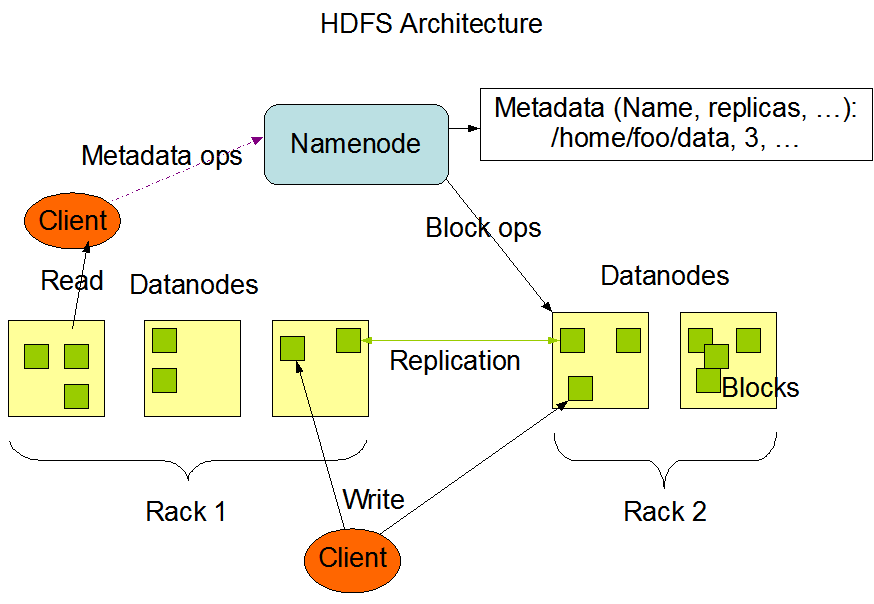
\includegraphics[width=120mm]{hdfsarchitecture.png}
\caption{HDFS Architecture (hadoop.apache.org)}
\label{fig:hdfs}
\end{center}
\end{figure}

While a normal filesystem manages files contained on a specific disk, HDFS treats the combined sum of all the storage of all the nodes attached to the system as a single disk. Files then live somewhere on the cluster, with redundancy such that all files can be replicated to a variable number of nodes. To achieve this Hadoop operates a single NameNode, combining the remainder of the cluster into DataNodes. The NameNode is responsible for keeping track of which system a given file lives on. The current implementation keeps all files available on the system in memory. There is optionally a secondary namenode which is tracking the changes in case the primary fails. The minimum block size on the system is set unusually high for a file system, on the order of 64 Megabytes. This means an extremely large file may have 64MB chunks all over the system, with each chunk replicated to possibly two or mode nodes. The DataNodes each manage read/write requests to the chunks that they control. The design decisions were driven by the need to quickly and efficiently partition a large data set and stream the input to the various Mappers. In addition, Hadoop is optimized for data locality, meaning that computation is designed to happen where the data is already residing. This assumes that it is cheaper to launch additional mappers where data is being stored, then to transfer the data to a fixed number of mapper instances, which is the case when processing the huge amounts of data in todays systems. 

\subsection{Hadoop MapReduce}
Hadoop MapReduce is based off the system described by the Google paper \cite{mapreduce}. Again like GFS, we don't have the actual Google implementation, so most descriptions of distributed MapReduce are going to be about the Hadoop model. MapReduce is, in itself, extremely simple. The subtlety in the system is how it accomplishes simplicity while continuing to scale to huge data amounts. MapReduce can be described in two ways, first a definition of the MapReduce pipeline, and second by the interfaces that an application developer need to implement in order to submit jobs to a Hadoop cluster. First, MapReduce contains 

\begin{itemize}

\item A Map step. In this step tuples are streamed off the storage device, each tuple being run through a single mapper. The mapper may output any number of tuples, either identified by any number of keys. 

\item A shuffle step. In this step the outputs from the mappers are sorted. This is to allow all tuples of the same key to be sent to the same reducer. 

\item An optional reduce step. In this step all tuples with the same key are run through the reducer. The reducer may output a new tuple using the same key as was input. This step is optional because there exists a Null reducer, which simply stores the output of the map step as an output of the whole algorithm. A second way to visualize MapReduce is from the interfaces provided by the Hadoop API. 

\end{itemize}
From this description it is hard to imagine what kinds of jobs can be framed in the MapReduce context. Problems which have a natural MapReduce implementation are ones that involve streaming over a large data set a single time. Examples of this include problems like counting, averaging, computing Min/Max, performing some transformation over a data set perhaps by normalizing multiple input formats into the same format. Some these jobs may not even require a reduce step, which is in fact optional. In this case, aside from job configuration there are two important interfaces. 


\begin{lstlisting}[label=some-code,caption=Mapper Interface]
public class MyMapper<K extends WritableComparable,
                      V extends Writable> 
  extends MapReduceBase implements Mapper<K, V, K, V> {
       
  public void map(K key, V val,
                  OutputCollector<K, V> output, 
                  Reporter reporter) { 
   }
\end{lstlisting}

\begin{lstlisting}[label=some-code,caption=Reducer Interface]
public class MyReducer<K extends WritableComparable,
                       V extends Writable> 
   extends MapReduceBase implements Reducer<K, V, K, V> {
       
   public void reduce(K key, Iterator<V> values,
                      OutputCollector<K, V> output, 
                      Reporter reporter) {
   }
\end{lstlisting}

The interfaces both deal with keys and values. In order for a mapper or reducer to output tuples they interact with the Reporter class. The shuffle step mentioned in the previous description is hidden from the application developers view and handled by the Hadoop layer. Here the key distinction between Mappers and Reducers can be highlighted in that Mappers take a single key and a single value per invocation while the reducers take a key along with an iterator of all the values (potentially very many) that match that particular key. 

\section{Parallel Models}
A number of models have been introduced to aid in reasoning about parallel programs and to bound efficiency for parallel algorithms. These models have enjoyed success in discriminating between problems that are efficiently parallelizable and problems that are "likely sequential". It will be important when defining any computational model which describes MapReduce to be able to compare and contrast the power of the MapReduce model to the power of the other parallel models like PRAMs and BSPs. Unfortunately, the model presented by MapReduce is different then any theoretical model studied to date. To that end a short description of those classes and models is included here, and the central result, which is the definition of the class NC and its distinction from P-Complete is discussed. 
 
\subsection{PRAM}
The Parallel Random Access Machines (PRAM) model has been the most successful and widely studied of the parallel computing models. A RAM machine is a natural extension of a Turing Machine that behaves similarly to a modern CPU based computer. It has a Random access memory and can execute a set number of natural instructions, including add, load, store, subtract. It enjoys a polynomial simulation relationship with regular tape based Turing Machines \cite{ram}.

A PRAM is a parallel extension of a RAM that models multiple RAMs hooked into the same memory bus. This is diagrammed in Figure ~\ref{fig:pram} A modern example is a multicore CPU, but PRAMs were developed to help deal with, at the time, highly parallel supercomputers like those designed and built by Cray and SGI. One of the pivotal issues surrounding PRAMs is the resolution of simultaneous access to identical memory locations by different CPUs. MapReduce can obviates this particular issue because it does not support general purpose addressing. In particular each tuple is dealt with by one and only one Mapper, while the Reducer is only going see an (potentially ordered) list of tuples. In this model there is no direct memory sharing, the only communication that can happen is between tuples. On the surface this may appear to make PRAMs a more powerful model then any model describing MapReduce. This issue will reappear in a later section. 

\begin{figure}[h]
\begin{center}
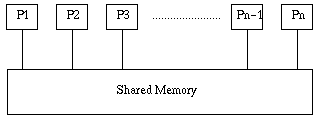
\includegraphics[width=120mm]{reportpram.png}
\caption{PRAM Architecture}
\label{fig:pram}
\end{center}
\end{figure}

The key relationship being studied under PRAMs, and any parallel model, is the relationship between the number of processors/systems required and the amount of input being processed. This will be further elaborated upon when describing NC, however we can say here that not all problems exhibit the same behavior when executed on a parallel machine. There are a number of problems when it comes to actually implementing PRAM systems. The primary problem being that connecting any number of CPUs to a central memory bus is problematic \cite{pram}. 

\begin{quotation}
In particular, a multiported memory which is shared by a large number of processors is infeasible. Instead a realistic and scalable parallel computer consists typically of a set of processor/memory module pairs which are connected by a sparse network of links. 
\end{quotation}

An initial approach to simplifing the realistic implementation of a PRAM machine is to reduce the number of interconnects between processors, instead connecting them into modules of fixed degree and the connecting the modules together. Another approach is to relax the communication requirements between processors, allowing them some autonomy in their computation and communicating only when necessary rather then at, potentially, each clock cycle. This is further explored in BSP.

Before we begin that section its worthwhile to ask the question, will it always be infeasible to connect a large number of processors to a shared bus? If the answer is no, and there is not in fact a theoretical problem with the construction of these machines, then there is always hope in the future that the engineering challenges will be solved and large scale parallel computing devices will be constructed that will {\bf not} require sparse interconnects between processors. Will these machines operate faster then any conceivable device which requires some kind of clustering? In fact Intel claims to have developed a single-chip cloud computer which 

\begin{quotation}
incorporates technologies intended to scale multi-core processors to 100 cores and beyond, such as an on-chip network, advanced power management technologies and support for “message-passing.” \cite{intel}
\end{quotation}

To answer this question requires the analysis of the performance characteristics of a MapReduce model to a PRAM model. First, without MapReduce, they would suffer from a difficult to implement parallel programming software model. And, of course even if these CPUs could be constructed, they could always be linked together using sparse network links to create even more powerful machines. In short MapReduce is likely to remain a viable framework even in the face of hardware improvements. 

\subsection{BSP}
The Barrier Sequential Parallel (BSP) Machine presents a modified view of parallel computing. In a PRAM, all the CPUs on the system are required to operate on a shared memory bus, and thus resolve coincident memory address on every single instruction cycle. BSPs take a different approach and instead operate in distinct cycles of {\bf processing} and {\bf communication}. They were originally introduced as a mechanism to reduce the complexity of parallel computing. 

\begin{quotation}
Some take the view that models based on shared memory are easier to program because
they provide the abstraction of a single, shared address space and so a whole class of placement
decisions are avoided. Moderately-parallel architectures capable of providing this abstraction
can certainly be built, so they also believe that the modest parallelism they provide is enough
to satisfy performance demands for the foreseeable future. We are dubious about both claims.
While shared memory does reduce the need for placement, it creates a need to control simul taneous access to the same location. This requires either careful crafting of programs, in
the PRAM style, or expensive lock management. Implementing shared-memory abstractions
requires a larger and larger fraction of the computer's resources to be devoted to communication and the maintenance of coherence. Worse still, the technology required to provide the
abstraction is the least likely to be of a commodity nature, and hence even more expensive.

The Bulk Synchronous Parallel (BSP) model provides software developers with an
attractive escape route from the world of architecture-dependent parallel software. \cite{bsp}

\end{quotation}


BSPs are interesting because they were originally developed as a simplification of the programming model presented by PRAMs. In particular there is a library extensions for numerous shared memory architectures that offer a simplified architecture. This library contains functions like bsp\_send and bsp\_move which send and fetch information from a particular processors queue, as well as bsp\_sync which synchronizes processors at a barrier. 

The model, while developed for shared memory systems, bares a striking similarity to the one offered by MapReduce. Both architectures have computation phases that are synchronized via communication. In BSP the communication is direct access from processor to processor, where in MapReduce communication is through tuples output. In BSP there are barriers at predefined locations and MapReduce operates in rounds. It is easy to imagine that MapReduce can efficiently simulate arbitrary BSP programs, and this will be mentioned further below.   

\subsection{NC}

Obviously one of the central areas of study of computer science and computation complexity over the past 30 years has been dividing up known problems into P or NP. Is the problem tractable, or not? Once this distinction has been made the problem quickly enters the realm of optimization. And over the past 50 years it seemed like increasing processing speeds would {\bf always} keep pace with input size. 

\begin{quotation}
So why don't we think PRAM anymore when we look at NC? Moore's Law. Processors got faster. Much much faster. The ideas of having many many processors each doing a tiny bit of work seems wasteful these days when we can just as cheaply have each processor do a lot of work. \cite{pramblog}
\end{quotation}

However, as data sizes have increased and sequential processors have faced ever diminishing returns, a question asked at least 15 years ago has come around again with increased importance. In particular

\begin{quotation}
Does every problem with a feasible sequential solution also have a feasible highly parallel solution? \cite{limits}
\end{quotation}

For this to make sense we need to define the term, highly feasible. For example, if a problem takes $T$ time to solve using a single processor, how long would it take to solve using $n$ processors. It would be nice if 
\[
\text{Time To Solve Using N Processors} = 
\frac{\text{Time To Solve Using 1 Processor}}{\text{N}}
\]

If a problem obeys this relationship, then its safe to say that the problem is highly parallel. Of course there will always be practical constraints to obtaining this bound. Latency between processor communication being the friction put upon maximum performance. But, is it even theoretically possible to achieve this kind of performance for all problems? 

Unfortunately, the answer it probably no, there are some algorithms that will never be effectivly implemented in parallel hardware. The class of problems this is true for is referred to as P-Complete. NC is a subset of P-Complete, although it has yet to be shown that a problem exists which is not in NC and still in P. An example of such a problem is maximal lexicographically independent set. This problem, which has a greedy algorithm demonstrates a solution which, as is yet know, cannot run efficiently in parallel. This is due to the algorithm keeping a list of items that it has examined before moving to the next step. This greedy approach means that any number of machines working in parallel to solve this problem would be unable to run without excessive communication between them. There are a large number of P-Complete problems, although there is some indication that a suitable powerful MapReduce model may be able to solve some of them. 

\section{Computational Models For MapReduce}
With the preliminaries out of the way we are ready to proceed to the issue of MapReduce performance. The are a number of important questions to consider. How can we formalize MapReduce in a manner which will allow us to reason about its performance? What are the relevant components of such a system? How will this system compare to the existing parallel models? Although this field is extremely new, there have been several attempts at such formalizations. 

There will be several common themes each model attempts to address. These will be, what is the complexity of a mapper, and a reducer. How is it defined. How is the concept of rounds introduced. That is running MapReduce multiple times, using the output of the one rounds reducer to feed the next rounds mapper. Is complexity 

\subsection{MUD}
One of the first attempts at formalizing a model involving MapReduce was involved the concept of streaming computations. This arises from the most natural application of Hadoop MapReduce which is the processing of log files. More specifically the authors describe a model for  massive, unordered, distributed (MUD) computation. From this arises a question, "can any function computable by a streaming algorithm also be computed by a MUD algorithm?" \cite{mud}.  

A streaming algorithm is an machine which operates over the entire data set, a single time and in some specific, predefined order, usually the order things are stored in on disk. The specific machine used for the streaming is limited to operate in poly-logrithmic space. For example processing log files ordered by timestamp on the disk to extract average number of page views is an example of a streaming algorithm. In many situations these algorithms can run on a single machine. However, when scalability comes into play the question becomes; can we achieve performance increases for an arbitrary streaming algorithm using MapReduce, which will split up the data set into an unordered distributed computation?

\begin{figure}[h]
\begin{center}
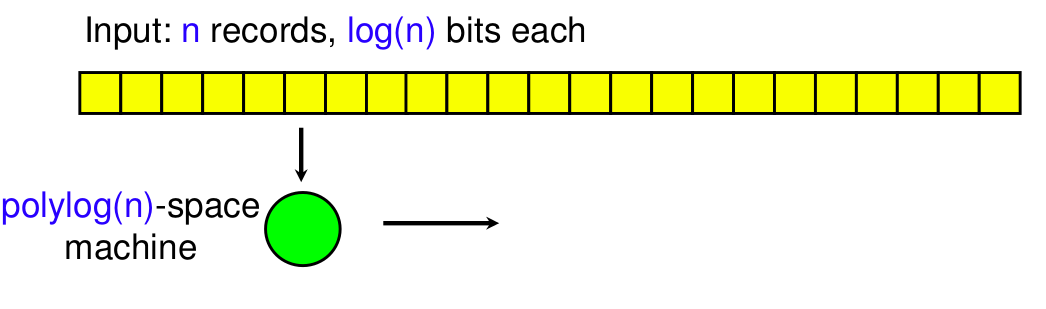
\includegraphics[width=120mm]{streaming.png}
\caption{Streaming Algorithms \cite{mud2}}
\label{fig:streaming}
\end{center}
\end{figure}


A mud algorithm is an abstraction upon symmetric stream algorithms with an eye towards distributed computation. There is nothing, however, explicitly parallel in their definition. Mud algorithms are defined to be a tuple ($\Phi, \oplus, \eta)$, where $\Phi$ maps input items to a message. $\oplus$ maps two message to a single message and $\eta$, which is a post-processor which maps a single message to an output state. The number of bits used to encode the message between these two jobs defines the communication complexity of the mud algorithm. In addition $\Phi, \oplus$, and $\eta$ all have space and time complexity measures. These items themselves, as described here, have no easily identifiable relationship to mappers and reducers. Only later will it become clear how these items are directly applicable to map reduce. Before we describe that though, we can note that even given this somewhat limited definition, we can already make some claims about the power of muds. 

\begin{figure}[h]
\begin{center}
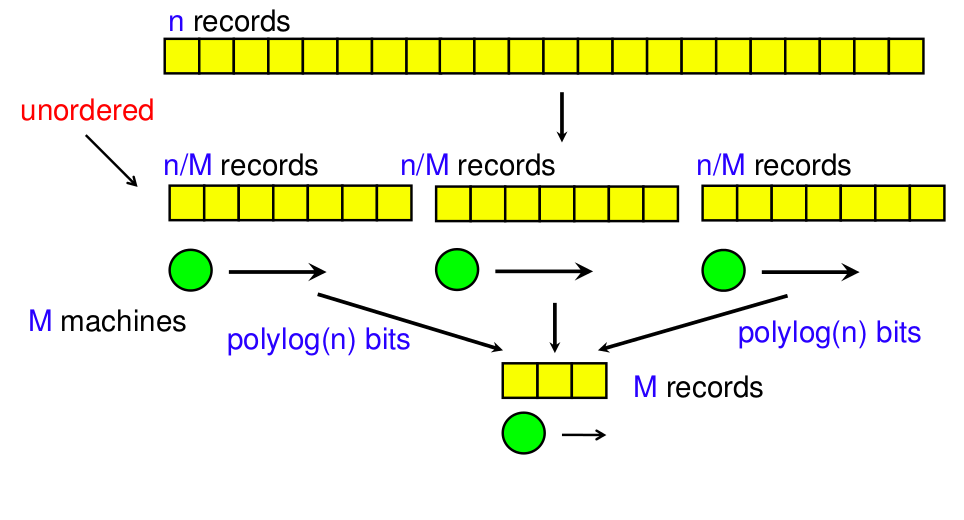
\includegraphics[width=120mm]{mud.png}
\caption{Mud Algorithms, an extension of streaming algorithms\cite{mud2}}
\label{fig:streaming}
\end{center}
\end{figure}

\subsubsection{Key Findings}

The authors are able to characterize the capabilities of MUDs very specifically. In particular, there exists a MUD algorithm to computer a symmetric streaming function $f$ if and only if $f$, 
\begin{itemize}
\item Is defined on all inputs
\item Has one unique output value
\item Has a streaming algorithm, which may be randomized through the use of public randomness. 
\end{itemize}

Symmetry is required in order to avoid edge case definitions of functions for which there can be no efficient mud algorithm. An example of this is computing an answer to the question "How many times does the first odd number appear in the output." \cite{mud2} This problem requires a total view of the input in order to compute, if each constituent $\Phi$ is is unable to know what the "first odd" number is, then it would be unable to count them over the input that it is processing. A normal streaming algorithm, as opposed to a symmetric one,  would have no issues with this problem definition. 

muds, by themselves, capture the essence of streaming computations. You could even view them as a different definition of symmetric streaming algorithms. However, some generalizations are required in order to capture all of the features of MapReduce. The authors go on to describe a multi-key mud, which is much more indicative of current MapReduce capabilities. A multi-key mud is a defined identically as a regular mud, consisting of $(\Phi, \oplus, \eta)$. In this definition $\oplus$ and $\eta$ remain the same and $\Phi$ is modified to produce input key,value In this context the $\Phi$ becomes a mapper and the $\oplus$ then becomes a reducer. Each mud operates on some subset of the input. There is still the idea of the $\eta$, which has no corresponding component in MapReduce. Also the the concept of "rounds" is introduced. This allows for multiple passes of data sets, each set using as input the output of the previous set. 

A key theorem using this distributed mud model can be stated as

\emph{Any problem in class NC has a polylog(n)-round, poly(n)-key mud algorithm with communication complexity
O(log(n)) bits per key.} 

This theorem is basically saying that for any problem in NC, there is an efficient (polylog) mud algorithm. The simulation shown, for which similar ideas will appear elsewhere, is to use one round of mud to simulate a single clock tick of a PRAM. Each $\Phi$ will process the output from a single processor and the $\oplus$ are responsible for resolving memory writes. 

There are some criticisms of this particular model. In particular, the power of the reducers seems to be artificially limited. This will be addressed by future models. Trying to use $\Phi$ and $\oplus$ to define a limited functionality framework which is extended to cover the MapReduce model, means that the mapping between the two paradigms is more abstract then it needs to be. In addition, simulations of more powerful machines are somewhat impractical. The authors put it succinctly, 

\begin{quotation}
Unfortunately, our simulation does not immediately provide a practical algorithm for obtaining speedups from distributing streaming computations over multiple machines because of the running time needed for the simulation, and for any specific streaming computation, alternative mud algorithms may be faster. \cite{mud}
\end{quotation}

This is not to say this model is without merit. Since streaming computations seem to be the most naturally suited to MapReduce, this model may be the most accurate in describing algorithms which would benefit from a MapReduce treatment. Later extensions to this model increase the power of the models, but perhaps expand their power beyond what is practically achievable using simple mappers and reducers. 

\subsection{MRC}
The Map Reduce Class model described in \cite{mrc} is a more direct approach to defining a model for MapReduce. In making this definition, the authors define a mapper and reducer function. Here a mapper is a function that takes as input a single tuple and outputs a multiset of new tuples. A reducer takes as input a key and a list of values for that key. It outputs that key and a new set of values. These definitions are very analogous to that capabilities of mappers and reducers in MapReduce. To that end both mappers and reducers can be viewed as either functions, or alternatively RAMs which can compute those functions. 

The authors can then take these definitions to provide a very concrete definition for problems solvable by MapReduce. An algorithm is in $MRC^i$ if there exists 
\begin{itemize}
\item A mapper, implemented by a RAM, that runs in $O(n^{1-e})$ space and polynomial time. 
\item A reducer, implemented by a RAM that runs in the same
\item A Total limitation on the total number of tuples to $O(n^{2-2e})$ 
\item A number of rounds R = $O(\log^i n)$
\end{itemize}

This model is different from muds in the following two ways. First, it enforces no ordering on the reducers. In the mud model, since it was based off of a streaming system, all the reducers operated one tuple at a time. In this model, each reducer can operate as it so chooses on all of the values for a given key. Second the computational restrictions on the reducer are also different. Specifically MUDs reducers ($\oplus$) are defined to operate in polylograthmic space. In MRC, reducers are allowed sublinear time and space. This provides MRC with more power. 

One of the interesting outcomes from this definition is that MRC contains some problems \emph{not} in NC (assuming that $P \ne NC$ which has not been proven). In particular the problem Padded Circuit Value, a modification of Circuit Value, is in MRC, and not in NC. This is because reducers are powerful enough by themselves to compute solutions to problems not in NC. And furthermore, the authors demonstrate, via a PRAM simulation that a large subset of problems in NC are also in MRC. The PRAM simulation is very similar to the one used for muds. 

\begin{quotation}
Conceptually,
we will use the mappers to route memory requests and
ship the relevant memory bits to the reducer responsible
for the particular processor. Each reducer will then
perform one step of computation for each of the PRAM
processors assigned to it, write out memory updates,
and request new memory positions. \cite{mrc}
\end{quotation}

The problem with this approach is that by allowing such powerful reducers, showing an algorithm is in MRC, does not with any certainty seem to ensure speedup via increased hardware resources. If all of the work in the algorithm is being done by a single reducer, there is no way to parallelize this algorithm without modifying the underlying algorithm. The approach taken by muds allows more certainty, since these algorithms are no more powerful then PRAMs.  


\subsection{MapReduce Framework} 
The MapReduce framework presented by Goodrich in his papers \cite{goodrich1}, \cite{goodrich2} probably go the longest way towards his stated goal of "putting the MapReduce framework on an equal theoretical footing with the well-known PRAM and BSP parallel models". This model, like MRC provides a direct relationship between the capabilities provided by MapReduce and the objects described by the model.

One of the key features of this model is that it is able to present an equation for lower bound computation time of an arbitrary MapReduce algorithm. For example, a given MapReduce round has a time cost described as,
\[
t_r + L + \frac{Cr}{B}
\]
For $t_r$ which denotes the maximum time taken by a mapper or reducer in round r, L which describes  the latency of the network. The is measured by the amount of time taken before a mapper or reducer receives its first message of input, and B which is the bandwidth of the shuffle network. And the parameter $C_r$ which describes the total communication complexity of round $r$. which is defined as the total number of inputs and outputs for all mapper and reducers. There are some interesting observations here. First note that if $C_r$ = B, in other words the shuffle network can operate as fast as the total number of tuples exported, then the cost of exporting those tuples drops to 1. In this case the running time of the MapReduce algorithm can entirely be described by the running time of the constituent mappers and reducers for all the rounds. If this is not the case, ie $C_r > B$, then there is an associated cost of shuffling the output of the mappers. Additionally, while L here is described as a constant, it is more likely a function of the input size. This is because there are practical constraints that arise as the number of mappers are increased. There is increased communication cost associated with spinning them up on the various systems, for example. These considerations are not really captured explicitly by the models previously mentioned. 

So while the other models place restrictions on the reducers I/O size, or require reducers to operate in a streaming fashion, this model allows maximum flexibility in their design. The total cost can include a number of factors as mentioned above, however the authors choose to focus on one particular measure, I/O buffer memory size.

Another feature introduced by these papers is a generic, graphical model which describes a MapReduce algorithm. This model is just another face on the MapReduce framework, in order to facilitate some different kinds of algorithm development and analysis. In this model mappers and reducers are represented by vertices. At program start time the input is used to initialize a certain subset of vertices with input. In each round edges are drawn between the vertices, representing communication that happens between the vertices. Once all the edges have been drawn for a given round, the process restarts itself, in the next round, with each vertex now using as input the output from the previous round. 

This model is handy because it is very aligned with the performance of a BSP. Therefore to simulate a BSP, create a vertex for each processor in the BSP. Each round is identical to a superstep of a BSP program. Communication, which is explicit in a BSP, is handled through the shuffle step in MapReduce. In this manner it is easy to show that any BSP which operates in R supersteps can be simulated by a MapReduce algorithm in R rounds. This framework also was proven to simulate an CRCW PRAM, the strongest kind of PRAM, in a logarithmic number of rounds with a $O(T(N+P) \log_(N+P))$ communications complexity for $T$ steps, $P$ processors, $N$ memory cells


\section{Open Questions}
 Will the computational models presented above ultimately be helpful in driving research and implementation towards larger, more efficient algorithms? Do the models presented above accurately capture the key elements of an arbitrary MapReduce program. There are definitely outstanding questions, regarding the relative power of MapReduce, which need to be answered. One of the primary questions is the precise relationship between NC and MapReduce. There seems to be evidence that MapReduce (with a certain definition) is more powerful then PRAMs when it comes to certain types of problems. This however doesn't help to define what precisely the difference between the classes. 

Another important practical question is what are the optimization tradeoffs when trying to implement MapReduce. There are a bunch of dials to adjust when creating algorithms. Guidance when making these decisions seems to be sparse at best. Some questions, applicable to any problem, include, 
\begin{itemize}
\item
What functions should the mapper perform. What functions should the reducer perform? What is the tradeoff of putting functionality in the mapper versus the reducer?
\item 
How many rounds should the algorithm take? Should the number of rounds be minimized, even at the expense of communication costs between the mappers/reducers?
\item
What is the format of the output of the mapper/reducer? How many tuples should the mappers be producing?
\item 
Where should intermediate results be placed? Should they be stored in a database, column store, distributed file system? How can complex algorithms, which may require multiple intermediate rounds, be managed. 
\end{itemize}

Each of the models presented above defines different approaches to answering the above questions. In MUD and MRC, the relative power of the reducer is limited, which encourages increased round cost. In the MapReduce Framework model these constituent components are not limited, but rather quantified. These creates a more expressive model, however does not assist when making algorithmic decisions. 

The graphical description of MapReduce presented in \cite{goodrich} is designed to provide an easier abstraction to developing algorithms. In this model, rather then worrying about specific functionality of mappers and reducers, input and output tuples, the developer can conceptually think of the steps of the algorithm as a evolving graph structure. It may even be possible to develop tools which will actually visualize the algorithm as it runs. The algorithms presented to compute prefix sums and also to simulate a BSP seem very straightforward when presented in this fashion, specifying vertices and edges rather then mappers and reducers. However, in this scheme after the initial round, mappers no longer provide any functionality and only pass tuples onto the reducers. This seems like a limited approach to algorithm development. And even assuming you can simulate an arbitrary BSP within the language of this model, the initial BSP algorithm still requires development. And, furthermore, there are no tools available to specify MapReduce programs in this model. A future area of development might be to develop a set of libraries which will allow algorithm developers to write programs using this approach, rather then going through the traditional MapReduce API presented earlier. 

\section{Conclusion}
MapReduce is an extremely important software framework, which will allow the analysis of ever increasing data sets. There is already a growing body of research investigating the details of the MapReduce paradigm, including underlying distributed file systems, and the specifics of mappers and reducers. MapReduce is not the first parallel distributed computational model studied. In particular PRAMS and BSP are both relevant when discussing the algorithmic characteristics of MapReduce. The research presented above attempts to present a theoretical framework in which to reason about relative MapReduce performance. There are several different approaches which attack the problem in a different fashion. The key features being described are, what is the relative power of mappers and reducers, how is the communications complexity going to be characterized, how do the number of rounds affect the power of the algorithms. 


\begin{thebibliography}{9}

\bibitem{cern}
  European Organization For Nuclear Research, 
  \url{http://public.web.cern.ch/public/en/lhc/Computing-en.html}.
  
\bibitem{dbms2}
DBMS2, eBay followup — Greenplum out, Teradata $>$ 10 petabytes, Hadoop has some value, and more, \url{http://www.dbms2.com/2010/10/06/ebay-followup-greenplum-out-teradata-10-petabytes-hadoop-has-some-value-and-more}.

\bibitem{facebook}
Namit Jain, \emph{Facebook’s Petabyte Scale Data Warehouse using Hive and Hadoop}, Facebook Data Infrastructure Team.

\bibitem{concurrency}
Herb Sutter, \emph{The Free Lunch Is Over: A Fundamental Turn Toward Concurrency in Software}, Dr Dobbs Journal, March 2005

\bibitem{intel}
Intel, \emph{From a Few Cores to Many}

\bibitem{mapreduce}
Jeffrey Dean and Sanjay Ghemawat, \emph{MapReduce: Simplied Data Processing on Large Clusters}, OSDI, 2004.

\bibitem{bigtable}
Fay Chang, Jeffrey Dean, Sanjay Ghemawat, Wilson C. Hsieh, Deborah A. Wallach
Mike Burrows, Tushar Chandra, Andrew Fikes, Robert E. Gruber, \emph{Bigtable: A Distributed Storage System for Structured Data}, OSDI, 2006.

\bibitem{gfs}
Sanjay Ghemawat, Howard Gobioff, and Shun-Tak Leung, \emph{The Google File System}, 19th ACM Symposium on Operating Systems Principles, Oct 2003.

\bibitem{hdfs}
Konstantin Shvachko, Hairong Kuang, Sanjay Radia, Robert Chansler, \emph{The Hadoop Distributed File System}, 2010.

\bibitem{intel}
Intel, \emph{	 Single-Chip Cloud Computer} , \url{http://techresearch.intel.com/ProjectDetails.aspx?Id=1}, 2010. 

\bibitem{lamport94}
  Leslie Lamport,
  \emph{\LaTeX: A Document Preparation System}.
  Addison Wesley, Massachusetts,
  2nd Edition,
  1994.

\bibitem{ram}
Stephan A Cook and Robert Reckhow, \emph{Time Bounded Random Access Machines}, Journal Of Computer and System Sciences, 1973. 

\bibitem{pramblog}
Lance Fortnow, \emph{What Happened to the PRAM}, \url{http://blog.computationalcomplexity.org/2005/04/what-happened-to-pram.html}, April 2005. 

\bibitem{pram}
Tim J Harris, \emph{A Survey Of PRAM Simulation Techniques}, ACM Computing Surveys, 1994. 

\bibitem{bsp}
D.B. Skillicorn, Jonathan M.D. Hill and W.F. McColl, \emph{Questions and Answers about BSP}, Nov 1996. 

\bibitem{limits}
Raymond Greenlaw, H. James Hoover, Walter L. Ruzzo, \emph{Limits to Parallel Computation: P-Completeness Theory}, OXFORD UNIVERSITY PRESS, 1995.

\bibitem{mud}
Jon Feldman, S. Muthukrishnan, Anastasios Sidiropoulos, Cliff Stein, Zoya Svitkina, \emph{On Distributing Symmetric Streaming Computations}, Sept 2009. 

\bibitem{mud2}
Anastasios Sidiropoulos (MIT), \emph{On Distributing Symmetric Streaming Computations}, \url{http://ttic.uchicago.edu/~tasos/papers/mud_soda2008_presentation.pdf}

\bibitem{mrc}
Howard Karloff, Siddharth Suri, Sergei Vassilivitskii, \emph{A Model Of Computation For MapReduce}, 
Symposium on Discrete Algorithms (SODA), 2010. 

\bibitem{goodrich1}
Michael T. Goodrich, \emph{Simulating Parallel Algorithm in the MapReduce Framework with Applications to Parallel Computational Geometry}, arxiv, April 27, 2010. 

\bibitem{goodrich2} 
Michael T. Goodrich and               Nodari Sitchinava and               Qin Zhang, 
\emph{Sorting, Searching, and Simulation in the MapReduce Framework}, arxiv, 2011. 

\end{thebibliography}

\end{document}
